\documentclass[a4paper,12px]{article}

\usepackage{graphicx}
\usepackage[english]{babel}
\usepackage{fancyhdr}
\usepackage{lastpage}
\usepackage{xifthen}
\usepackage[linesnumberedhidden, titlenotnumbered]{algorithm2e}
\usepackage{lipsum}
\usepackage{hyperref}
\usepackage{array}
\usepackage{tabularx}

\usepackage{minted}
\usepackage{caption}
\usepackage{amssymb}

\pagestyle{fancy}
\lhead{
\includegraphics[width=7cm]{logoUvA}}
\rhead{\footnotesize \textsc {Report\\ \opdracht}}
\lfoot
{
    \footnotesize \studentA
    \ifthenelse{\isundefined{\studentB}}{}{\\ \studentB}
    \ifthenelse{\isundefined{\studentC}}{}{\\ \studentC}
    \ifthenelse{\isundefined{\studentD}}{}{\\ \studentD}
    \ifthenelse{\isundefined{\studentE}}{}{\\ \studentE}
}
\cfoot{}
\rfoot{\small \textsc {Page \thepage\ of \pageref{LastPage}}}
\renewcommand{\footrulewidth}{0.5pt}

\fancypagestyle{firststyle}
{
    \fancyhf{}
    \renewcommand{\headrulewidth}{0pt}
    \chead{
\includegraphics[width=7cm]{logoUvA}}
    \rfoot{\small \textsc {Page \thepage\ of \pageref{LastPage}}}
}

\setlength{\topmargin}{-0.3in}
\setlength{\textheight}{630pt}
\setlength{\headsep}{40pt}

% =================================== DOC INFO ===================================

\newcommand{\titel}{GPGPU: CUDA}
\newcommand{\opdracht}{Assignment 5.1: Wave Equation}
\newcommand{\docent}{Dr. R.G. Belleman}
\newcommand{\cursus}{Concurrency and Parallel Programming}
\newcommand{\vakcode}{5062COPP6Y}
\newcommand{\datum}{\today}
\newcommand{\studentA}{Robin Klusman}
\newcommand{\uvanetidA}{10675671}
\newcommand{\studentB}{Maico Timmerman}
\newcommand{\uvanetidB}{10542590}
%\newcommand{\studentC}{Boudewijn Braams}
\newcommand{\uvanetidC}{10401040}
%\newcommand{\studentD}{Govert Verkes}
\newcommand{\uvanetidD}{10211748}
%\newcommand{\studentE}{Naam student 5}
\newcommand{\uvanetidE}{UvAnetID student 5}

% ===================================  ===================================

\begin{document}
\thispagestyle{firststyle}
\begin{center}
    \textsc{\Large \opdracht}\\[0.2cm]
    \rule{\linewidth}{0.5pt} \\[0.4cm]
    {\huge \bfseries \titel}
    \rule{\linewidth}{0.5pt} \\[0.2cm]
    {\large \datum  \\[0.4cm]}

    \begin{minipage}{0.4\textwidth}
        \begin{flushleft}
            \emph{Student:}\\
            {\studentA \\ {\small \uvanetidA \\[0.2cm]}}
            \ifthenelse{\isundefined{\studentB}}{}{\studentB \\ {\small \uvanetidB \\[0.2cm]}}
            \ifthenelse{\isundefined{\studentC}}{}{\studentC \\ {\small \uvanetidC \\[0.2cm]}}
            \ifthenelse{\isundefined{\studentD}}{}{\studentD \\ {\small \uvanetidD \\[0.2cm]}}
            \ifthenelse{\isundefined{\studentE}}{}{\studentE \\ {\small \uvanetidE \\ [0.2cm]}}
        \end{flushleft}
    \end{minipage}
    ~
    \begin{minipage}{0.4\textwidth}
        \begin{flushright}
            \emph{Supervisor:} \\
            \docent \\[0.2cm]
            \emph{Course:} \\
            \cursus \\[0.2cm]
            \emph{Course code:} \\
            \vakcode \\[0.2cm]
        \end{flushright}
    \end{minipage}\\[1 cm]
\end{center}


% =================================== FRONT PAGE ===================================

\vspace{2cm}
\begin{center}
    
\includegraphics[width=(\textwidth/5*3)]{parallel_tasks}
\end{center}
\clearpage

\tableofcontents
\vspace{5mm}

% =================================== MAIN TEXT ===================================

\section{Introduction}

For this assignment CUDA is used to simulate a wave equation. Indeed, this is a
program we have seen before, our aim then in this implementation will be to try
and increase the performance of this program by using CUDA.
CUDA uses the graphics processing unit to perform the same operation on a large
amount of data. The GPU is perfect for this task, since it has a large amount of
ALU's.

\section{Method}

The implementation of this program is fairly straightforward, we simply spread
the amplitude points over the available ALU's, each of which will calculate the
next value for that particular amplitude point. So we only need one iteration
per ALU per time step to compute the wave.

\section{Results}

In the results below it can be seen that CUDA has a significantly better
performance than the previous implementations of this program. This can be
explained partially by realising that CUDA has many more ALU's to its disposal
than any of the previous programs, which only used a maximum of eight parallel
threads to execute the program. CUDA on the other hand has access to over a
million total hardware threads, so it comes as no surprise that CUDA is faster
when computing this highly parallelisable wave simulation.

\begin{center}
    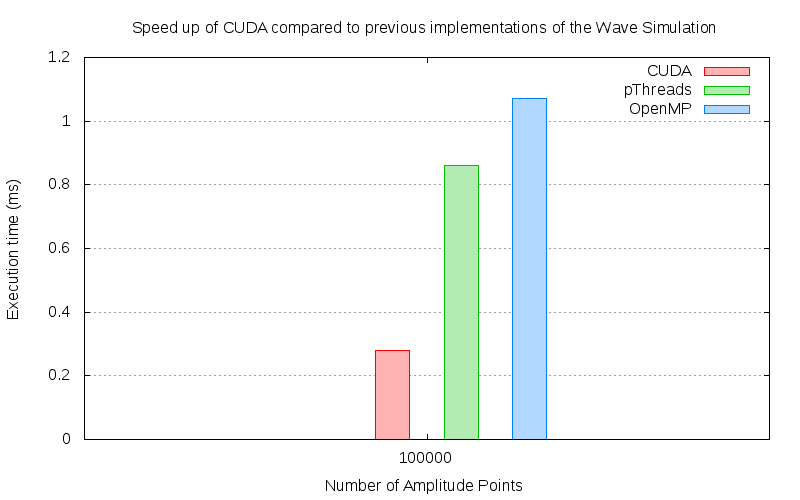
\includegraphics[width=\textwidth]{speedup01mil}
\end{center}
\captionof{figure}{Comparison of execution times (in seconds) of 10000 time steps in a wave of 100000
    amplitude points for CUDA, OpenMP (8 threads with dynamic scheduling) and
    pThreads (8 threads).}

\begin{center}
    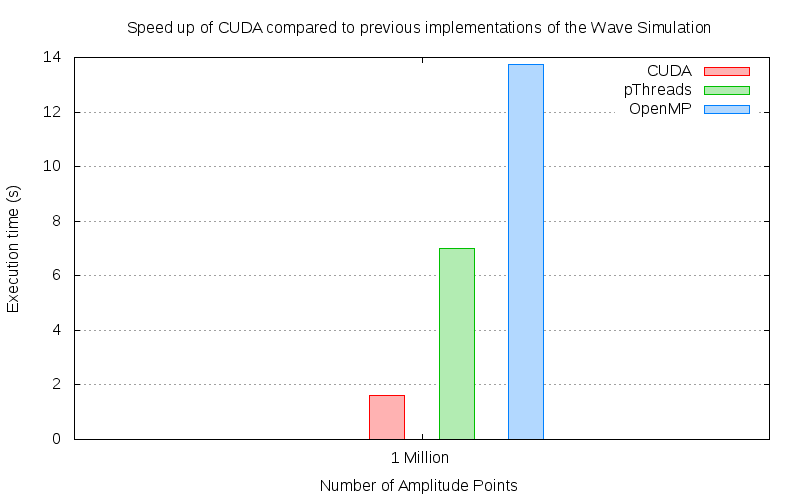
\includegraphics[width=\textwidth]{speedup1mil}
\end{center}
\captionof{figure}{Comparison of runtimes of 10000 time steps in a wave of 1
    million amplitude points for CUDA, OpenMP (8 threads with dynamic
    scheduling) and pThreads (8 threads).}

\begin{center}
    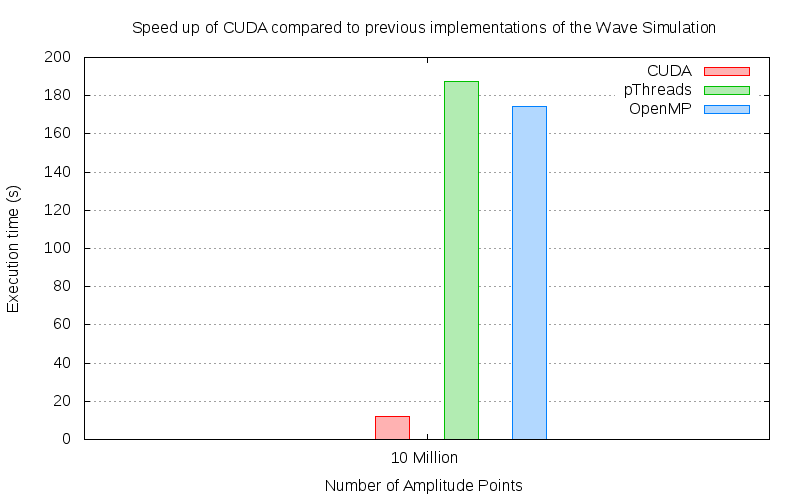
\includegraphics[width=\textwidth]{speedup10mil}
\end{center}
\captionof{figure}{Comparison of runtimes of 10000 time steps in a wave of 10
    million amplitude points for CUDA, OpenMP (8 threads with dynamic
    scheduling) and pThreads (8 threads).}

\section{Conclusion}

As stated above, it comes as no surprise that using CUDA is many times faster
than using any of the previous parallel programming options. CUDA of course has
access to a great many more ALU's than the other implementations do. Though when
comparing the execution in CUDA for 0.1 million amplitude points to 10 million
points, we see that CUDA does need significantly more time to compute those 10
million points, even though it still only needs one iteration (per time step) to
complete the simulation, due to the amount of cores being sufficient to
accommodate all the 10 million points. This extra overhead is then most likely
created by the extra time it takes to transport all this data.


% =================================== REFERENCES ===================================

%\clearpage
%\bibliographystyle{unsrt}
%\bibliography{bib}

\end{document}
